% !TEX encoding = UTF-8 Unicode
\documentclass[11 pt, a4paper,titlepage]{report}
%\documentclass[11pt, oneside]{memoir}   
\usepackage[margin=0.9in]{geometry}             

\RequirePackage{fix-cm}
\RequirePackage{titlesec}
\RequirePackage{titletoc}  

%% --------------- Load packages for large documents. ------------------
%% Hyperref is used to setup the hyperlinking between 
%% chapter/section/subsection and contents, citing and references,
%% and footnotes. \widowpenalty and \clubpenalty are used to suppress
%% WINDOWS (the last line of a paragraph typed as the first line of a 
%% new page) and ORPHANS (the first line of a paragraph as the last
%% line of a page).
\usepackage{chapterbib}
% For Bib by Chapter, bibtex the .aux file for each chapter after latex of main
%\usepackage{cite}%                %conflicting with hyperref
\usepackage[colorlinks,%
linkcolor=black,%
anchorcolor=black,%
citecolor=black]{hyperref}%         %setup hyderlinking
\widowpenalty=10000%
\clubpenalty=10000%                % suppress widows and orphans



%\renewcommand{\chaptername}{Chapter}
\titleformat{\chapter}[display]%
  {\bfseries\fontsize{16pt}{19.2pt}\selectfont}
  {\chaptertitlename\ \thechapter}{\baselineskip}{}
\titleformat{\section}[hang]%
  {\bfseries\fontsize{14pt}{16.8pt}\selectfont}
  {\thesection}{\baselineskip}{}
\titleformat{\subsection}[hang]%
  {\bfseries\fontsize{12pt}{14.4pt}\selectfont}
  {\thesubsection}{\baselineskip}{}
  
  
\usepackage{array}
\usepackage{amssymb}
\usepackage{amsmath}
\usepackage{caption}

\usepackage{rotating}
\usepackage{chapterbib}
\usepackage{graphicx}	
\usepackage{ctable}
\usepackage{multirow}
\usepackage[normalsize]{subfigure} 										
	

%% This is for the code segments of manual!!
\usepackage{color}
\usepackage{listings}
\lstdefinestyle{ MyBash}{language=bash,                % choose the language of the code
basicstyle=\footnotesize,       % the size of the fonts that are used for the code
numbers=left,                   % where to put the line-numbers
numberstyle=\footnotesize,      % the size of the fonts that are used for the line-numbers
stepnumber=1,                   % the step between two line-numbers. If it is 1 each line will be numbered
numbersep=5pt,                  % how far the line-numbers are from the code
backgroundcolor=\color{white},  % choose the background color. You must add \usepackage{color}
showspaces=false,               % show spaces adding particular underscores
showstringspaces=false,
commentstyle=\color{red},
keywordstyle=\color{blue},
showtabs=false,                 % show tabs within strings adding particular underscores
frame=single,           % adds a frame around the code
tabsize=2,          % sets default tabsize to 2 spaces
captionpos=b,           % sets the caption-position to bottom
breaklines=true,        % sets automatic line breaking
breakatwhitespace=false,    % sets if automatic breaks should only happen at whitespace
escapeinside={\%*}{*)}          % if you want to add a comment within your code
}

\lstdefinestyle{MyCpp}{ language=C++,                % choose the language of the code
basicstyle=\footnotesize,       % the size of the fonts that are used for the code
numbers=left,                   % where to put the line-numbers
numberstyle=\footnotesize,      % the size of the fonts that are used for the line-numbers
stepnumber=1,                   % the step between two line-numbers. If it is 1 each line will be numbered
numbersep=5pt,                  % how far the line-numbers are from the code
backgroundcolor=\color{white},  % choose the background color. You must add \usepackage{color}
showspaces=false,               % show spaces adding particular underscores
showstringspaces=false,
basicstyle=\ttfamily,
keywordstyle=\color{blue}\ttfamily,
stringstyle=\color{red}\ttfamily,
commentstyle=\color{green}\ttfamily,
morecomment=[l][\color{magenta}]{\#},
showtabs=false,                 % show tabs within strings adding particular underscores
frame=single,           % adds a frame around the code
tabsize=2,          % sets default tabsize to 2 spaces
captionpos=b,           % sets the caption-position to bottom
breaklines=true,        % sets automatic line breaking
breakatwhitespace=false,    % sets if automatic breaks should only happen at whitespace
escapeinside={\%*}{*)}          % if you want to add a comment within your code
}


\usepackage{fancyhdr}

%\setlength{\droptitle}{-5em}   % This is your set screw
\usepackage[parfill]{parskip}
\setlength{\parskip}{1pt}
\setlength{\parsep}{1pt}
\setlength{\topsep}{0pt}
\setlength{\partopsep}{0pt}

\graphicspath{ {./figures/} }

\pagestyle{fancy}
\fancyhf{}
\fancyhead[R]{ PB-[S]AM manual}
\fancyfoot[R]{\thepage\ }



\renewcommand\contentsname{Table of Contents}



\newcommand{\param}[1]{$\textless\texttt{#1}\textgreater$}
\newcommand\T{\rule{0pt}{3.0ex}}       % Top strut
\newcommand\B{\rule[-2ex]{0pt}{0pt}}


%%%%%%%%%%%%%%%%%%%%%%%%%%%%%%%%%%%%%%%%%%%%%%%%%%%%%%%%%%%%%%%%%%
%%%%%%%%%%%%%%%%%%%%%%%%%%%%%%%%%%%%%%%%%%%%%%%%%%%%%%%%%%%%%%%%%%


\begin{document}



\begin{titlepage}
\pagenumbering{gobble}
\begin{center}
\vspace{5pt}

%\title
	{\huge \textbf{Reference Manual}}\\ 
	\vspace{0.2cm}
	{\huge Poisson Boltzmann Analytical Model (PB-AM)}\\ 
\vspace{5pt}

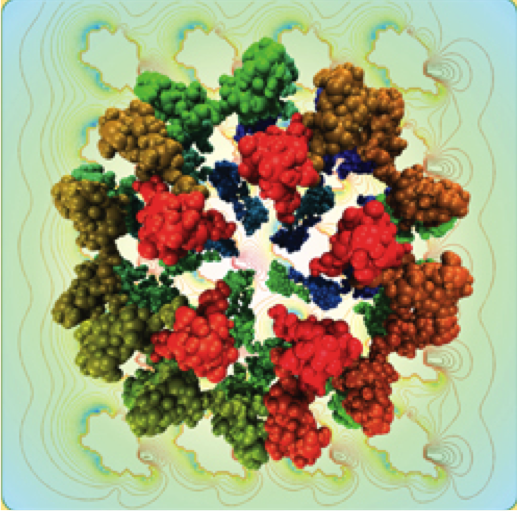
\includegraphics[scale=0.8]{cover}

%\author
	Enghui-Yap\\  
	Albert Einstein College of Medicine\\ 
\vspace{5pt}	
	
	Lisa Felberg\\ 
	Marielle Soniat\\
	David Brookes \\ 
	Teresa Head-Gordon\\ 
	University of California, Berkeley  
\vspace{5pt}

For more information, please visit http://thglab.berkeley.edu \\
\vspace{5pt}
\end{center}
\end{titlepage}



\textbf{Cover Illustration:} An exploded view of a Brome Mosaic Virus capsid 
composed of T = 1 particles (PDB: 1YC6), 
represented as collections of overlapping spheres, is shown. 
PB-SAM is a new semi-analytical approach to efficiently solve the 
linearized Poisson?Boltzmann equation using multipole formalisms for overlapping spheres. 
The background shows the potential profile for an array of 601YC6 monomers computed using this method. \\



\textbf{Recommended Citations:} \\

When citing PB-AM in the literature, the following citation should be used

I. Lotan and T. Head-Gordon (2006). An analytical electrostatic model for salt screened interactions between multiple proteins  J. Chem. Theory Comput 2, 541-555. \\ 


When citing PB-SAM in the literature, the following citations should be used

1.  E.-H. Yap and T. Head-Gordon (2010). New and efficient Poisson-Boltzmann solver for interaction of multiple proteins  J. Chem. Theory Comput. (Journal cover) 6, 2214-2224.

2.  E.-H. Yap and T. Head-Gordon (2013). Calculating the bimolecular rate of protein?protein association with interacting crowders.  J. Chem. Theory Comput. 9(5), 2481-2489.

3.   O. N. Demerdash, E.-H. Yap and T. Head-Gordon (2014). Advanced potential energy surfaces for condensed phase simulation.  Ann. Rev. Phys. Chem. 65, 149-174.   \\



\textbf{Acknowledgments:} Research support from NIH and DOE is gratefully acknowledged. \\


\tableofcontents

\pagenumbering{arabic}
\setcounter{page}{1}


\chapter{Introduction}

The Poisson-Boltzmann Analytical and Semi-Analytical models solve the linearized Poisson-Boltzmann Equation 
(PBE) for systems hitherto not possible using traditional PBE solvers. This manual describes 
the methods and their associated suite of programs. We will refer to each method by their acronyms:
PB-AM and PB-SAM. There is much shared capability between the two softwares, so when an application
or usage can be applied to both, we will refer to both of them as PB-[S]AM, with the S in square brackets.
The PBE software suite is licensed as a collection of freely available program under a GPL license. 


\section{PB-AM} The first general analytical solution for computing the screened electrostatic 
interaction between large numbers of macromolecules of arbitrarily complex charge distributions, 
assuming they are well described by spherical low dielectric cavities in a higher dielectric 
medium in the presence of a Debye-H{\"u}ckel treatment of salt. The method exploits 
multipole expansion theory for the screened Coulomb potential such that it can describe direct 
charge-charge interactions and all higher-order cavity polarization effects between low dielectric 
spherical cavities containing their charges, while treating these higher order terms correctly 
at all separation distances. The analytical solution is general to arbitrary numbers of 
macromolecules, is efficient to compute, provides for the first time the ability to provide new 
benchmarks for other numerical solutions to the linearized Poisson-Boltzmann equation. A 
number of utilities are described below that use PB-AM results.

\section{PB-SAM} 

A semi-analytical extension of the PB-AM method. It too is capable of computing the interactions
of multiple molecules with complex charge distributions, but because of its semi-analytical approach, 
molecules are now represented as a collection of overlapping spheres. This allows for a more complex
description of the molecule in comparison to the analytical method. The applications below also apply to the 
semi-analytical method.

\section{Physical Calculations} The PB-[S]AM results allow for fast calculation of physically important quantities. 
Specifically this program can calculate the interaction energy of, and the force and torque 
applied to each molecule. These results may be written into a file or printed to the terminal.

\section{Brownian Dynamics} This package also implements dynamics simulations using the 
Brownian protocol developed by Ermak and McCammon\footnote{Ermak, D. L.; McCammon, J. A. \textit{J. Chem. Phys.} 
1978, \textit{69}, 1352\---1360.}. At each time step, the translation and rotation due to the applied 
force and torque, respectively, are calculated and added to random components of motion. The user can specify 
spatial and temporal termination conditions for the simulation and write the trajectory to specified files.

\section{Electrostatics} Another possible output of PB-[S]AM, the user can specify a configuration of an 
arbitrary number of molecules and get a 2-dimensional or 3 dimensional potential landscape of the 
system. We have provided example plotting tools, and the 3-dimensional output may be 
uploaded in VMD for visualization.

\clearpage

\chapter{Theory}



\section{PB-AM formulation}

PB-AM is an analytical solution to the linearized Poisson-Boltzmann equations for multiple spherical objects of arbitrary charge distribution in an ionic solution.  The linearized Poisson-Boltzmann equation is given as:

\[ \nabla [\epsilon(r) \nabla\phi(r)] - \epsilon(r) \kappa^2\phi(r) = 4 \pi \rho(r) \] %∇[ϵ(r)∇Φ(r)]-ϵ(r) κ^2 Φ(r)=4πρ(r)

\[ \phi_{out}^{(i)}= \phi_{out}^{(i)} \biggr |_{r=a_i } \]

\[\epsilon_s \frac{\partial \phi_{out}^{(i)}}{\partial r} =   \epsilon_s \frac{\partial \phi_{out}^{(i)}}{\partial r} \biggr |_{r=a_i } \]

Exploiting fast-multipole methods, this boundary value problem can be reduced to the following system of linear equations.  

\[ A = \Gamma \cdot (\Delta \cdot T \cdot A + E) \]

A(i) represents the effective multipole expansion of the charge distributions of molecule (i). E(i) is the free charge distribution of molecule (i). $\Gamma$ is a dielectric boundary-crossing operator, $\Delta$ a cavity polarization operator, T an operator that transforms the multipole expansion to a local coordinate frame.  More details on the method are available in Lotan, Head-Gordon (2006). \\

\subsection{Physical Calculations}

From the above formulation, computation of the interaction energies ($\Omega^{(i)}$) is given as follows:

\[\Omega^{(i)}=\frac{1}{\epsilon_s} \left \langle \sum_{j \ne i}^N  T \cdot A^{(j) } ,  A^{(i) } \right \rangle \]

Where $\langle  M, N \rangle$ denotes the inner product. When energy is computed, forces follow as:

\[ \textbf{F}^{(i)} = \nabla_i \Omega^{(i)}=\frac{1}{\epsilon_s} [ \langle \nabla_i \,T \cdot A^{(i) } ,  A^{(i) } \rangle +  \langle T \cdot A^{(i) } ,   \nabla_i \, A^{(i) } \rangle ]\]


% Additonally, the torque $\tau^{(i)}_j$ on molecule $i$ due to a charge $q^{(i)}_j$ is calculated as follows:
The method to calculate the torque $\boldsymbol{\tau}^{(i)}$ on molecule is outside the scope of this manual, but is discussed extensively in Lotan, Head-Gordon (2006).

\subsection{Brownian Dynamics}

Brownian dynamics simulations are implemented by treating each molecule as a Brownian particle experiencing a conservative force $\textbf{F}^{(i)}$ and torque $\boldsymbol{\tau}^{(i)}$, as well as friction and random force due to the solvent. The translation $\Delta r_i$ and rotation $\Delta \theta_i$ for a time step $\Delta t$ are then given by

\[\Delta r^{(i)} = \frac{D_{i, trans} \Delta t}{k_B T} \textbf{F}^{(i)} + \textbf{S}_i(\Delta t)\]
\[\Delta \theta^{(i)} = \frac{D_{i, rot} \Delta t}{k_B T} \boldsymbol{\tau}^{(i)} + \boldsymbol{\Theta}_i(\Delta t)\]

where $D_{i, trans}$ and $D_{i, rot}$ are the translation and rotational diffusion coefficients for molecule $i$, respectively and $\textbf{S}_i(\Delta t)$ and $\boldsymbol{\Theta}_i(\Delta t)$ are the stochastic components of translation and rotation, respectively, which have the following properties:

\[\langle \textbf{S}_i \rangle=0, \qquad \langle \textbf{S}_i^2 \rangle=2D_{i, trans}\Delta t\]
\[\langle \boldsymbol{\Theta}_i \rangle=0, \qquad \langle \boldsymbol{\Theta}_i^2 \rangle=2D_{i, rot}\Delta t\]

\subsection{Electrostatics}

In a similar manner to the interaction energy calculations in the Physical Calculations section, the electrostatics computes the potential at any point in space exterior to the molecules, \textbf{r}, as the inner product of all the solved effective multipole expansions \(A^{(j)}\) with a local multipole expansion of a single positive charge at position, \textbf{r}.

\[\Phi_{out}(\textbf{r})= \frac{1}{\epsilon_s} \left \langle \sum_{j = 1}^N  T \cdot A^{(j) } , \,  A(\textbf{r})  \right \rangle \]

\clearpage


\chapter{Use}

\section{Installation}

To install this program, first download the source code from the GitHub repository: \\

\hspace{1cm}\texttt{\$ git clone https://github.com/davas301/pb\_solvers.git clone\_dir} \\

Then navigate to the cloned directory \texttt{clone\_dir}. From here, make a \texttt{build} directory, use CMake to create a make file and then make the program.  This is done as follows: \\

\hspace{1cm}\texttt{\$ cd clone\_dir} 

\hspace{1cm}\texttt{\$ mkdir build}

\hspace{1cm}\texttt{\$ cd build}

\hspace{1cm}\texttt{\$ cmake ..} 

\hspace{1cm}\texttt{\$ make pbam} \\

An executable named \texttt{pbam} will now be in \texttt{clone\_dir/build/bin}.

%%%%%%%%%%%%%%%%%%%%%%%%%%%%%%%%%%%%%%%%%%%%%%%%%%%%%%%%%%%%%%%%%%
%%%%%%%%%%%%%%%%%%%%%%%%%%%%%%%%%%%%%%%%%%%%%%%%%%%%%%%%%%%%%%%%%%
\section{Input Information}

\subsubsection{Input Files}

The program executable requires an input file as a command line parameter. The input file contains the various arguments and parameters that one may wish to set when running the program. Each line of the input file contains a keyword followed by a variable number of whitespace-delimited parameters, e.g.: \\

\texttt{keyword1\qquad param1\qquad param2} \\
\texttt{keyword2\qquad param1\qquad param2\qquad param3} \\

Each keyword is described in the table below, along with its associated parameters.


\newcommand{\param}[1]{$\textless\texttt{#1}\textgreater$}
\newcommand\T{\rule{0pt}{3.5ex}}       % Top strut
\newcommand\B{\rule[-2ex]{0pt}{0pt}}

\newlength{\colthree}
\setlength{\colthree}{10.1cm}
\newlength{\coltwo}
\setlength{\coltwo}{2.9cm}

\begin{tabular}{ c | l | l  }
    \textbf{Keyword} & \textbf{Parameters} & \textbf{Description} \\ \hline
\T runname & \param{name} & \parbox[t]{\colthree}{\param{name} is desired internal name of this run.} \\
\T attypes & \param{numtypes} & \parbox[t]{\colthree}{Set the number of different atom types to \param{numtypes}.}\\
\T pqr & \param{idx} \param{fpath} & \parbox[t]{\colthree}{The molecule index for this xyz file. Provide input PQR file at \param{fpath}.} \\
\T xyz & \param{idx} \param{fpath} & \parbox[t]{\colthree}{The molecule index for this xyz file. Provide input XYZ file at \param{fpath}.} \\
\T transrot & \param{idx} \param{fpath} & \parbox[t]{\colthree}{The molecule type index for this translation/rotation file that can be input instead of a xyz file. Provide input file at \param{fpath}.}\\
\T randorient &  & \parbox[t]{\colthree}{If you want your molecules to be randomly rotated, use this flag} \\
\T units & \param{units} & \parbox[t]{\colthree}{Set the units of output to \param{units}. The current options are: \texttt{jmol} (Joules/mole), \texttt{kT} and \texttt{kcalmol} (kCal/mole).}\\
\T salt & \param{con} & \parbox[t]{\colthree}{Set salt concentration in the system to \param{con}.}\\
\T temp & \param{T} & \parbox[t]{\colthree}{Set system temperature to \param{T}}\\
\T idiel & \param{ival} & \parbox[t]{\colthree}{Set the interior dielectric constant to \param{ival}.} \\
\T sdiel & \param{sval} & \parbox[t]{\colthree}{Set the solvent dielectric constant to \param{sval}.} \\
\T pbc & \param{boxlength} & \parbox[t]{\colthree}{Set size of periodic box to \param{boxlength}.}\\
\T random & \param{seed} & \parbox[t]{\colthree}{Seed the internal random number generator with \param{seed}.} \\
\T type & \parbox[t]{\coltwo}{\param{idx} \param{ct} \param{movetype} \param{dtr} \param{drot}} & \parbox[t]{\colthree}{Set attributes of an atom type, where \param{idx} is the integer id of this type, which can be 1 to \param{numtypes} (above). \param{ct} is the number of atoms of this type in the system and \param{movetype} describes the way this type is allowed to move in a dynamics run (\texttt{move}, \texttt{rot}, or \texttt{stat}). If \param{movetype} is \texttt{move}, then a translational diffusion coefficient \param{dtr} and a rotational diffusional coefficient \param{drot} are required. If \param{movetype} is \texttt{rot} then just \param{drot} is required. \B}\\
\hline
\end{tabular}


\setlength{\colthree}{8.1cm}
\setlength{\coltwo}{2.5cm}

\begin{tabular}{ c | l | l}
    \textbf{Keyword} & \textbf{Parameters} & \textbf{Description} \\ \hline

\T runtype electrostatics & \param{gridpts} & \parbox[t]{\colthree}{Will run electrostatics calculations. \param{gridpts} is an optional integer describing the number of evenly spaced points in each dimension to perform calculations on.\B}\\

\T dx & \param{fname} & \parbox[t]{\colthree}{For electrostatics. Will write the results of electrostatics calculations for every 3D grid point to \param{fname}, in the same output format as APBS dx file.\B} \\

\T 3dmap & \param{fname} & \parbox[t]{\colthree}{For electrostatics. Will write the results of electrostatics calculations for points on the surface of the molecules in the system.\B} \\

\T gridct & \param{ct} & \parbox[t]{\colthree}{For electrostatics. \param{ct} is the number of 2D grids to output.\B} \\

\T grid2d & \parbox[t]{\coltwo}{\param{idx} \param{fname} \param{axis} \param{val} } & \parbox[t]{\colthree}{For electrostatics. Set attributes of a grid output where \param{idx} is the integer id of this grid, which can be 1 to \param{ct} (above). Will write output of calculations for a cross section along \param{axis} (\texttt{x}, \texttt{y}, or \texttt{z}) at \param{value}.\B} \\

\hline
  \end{tabular}
  
  
  \begin{tabular}{ c | l | l}
    \textbf{Keyword} & \textbf{Parameters} & \textbf{Description} \\ \hline
\T runtype dynamics & \parbox[t]{\coltwo}{ \param{outname}  \param{ntraj}} & \parbox[t]{\colthree}{Will perform a brownian dynamics run. A directory where trajectory information will be stored in and the number of trajectories is required.\B}  \\

\T termct & \param{ct} & \parbox[t]{\colthree}{Set number of termination conditions to \param{ct}.}  \\

\T termcombine & \param{andor} & \parbox[t]{\colthree}{Set how termination conditions will be combined. \param{andor} should be \texttt{and} or \texttt{or}. Default is \texttt{or}.} \\

\T term & \parbox[t]{\coltwo}{\param{idx} \param{type} \param{val} \param{mols}} & \parbox[t]{\colthree}{Set attributes of a termination condition where \param{idx} is the integer id of this condition, which can be 1 to \param{ct} (above). \param{type} can be \texttt{time},  \texttt{x<=}, \texttt{y<=}, \texttt{z<=}, or \texttt{r<=} (or the \texttt{>=} equivalents of these), \param{val} is the value where the simulation will terminate and \param{mols} is a whitespace-delimited list of molecular indices that this condition applies to (\texttt{time} requires 0, and all else require 1). \B} \\

\T term \param{idx} contact & \parbox[t]{\coltwo}{\param{confile} \param{pad}} & \parbox[t]{\colthree}{Set attributes of contact termination condition, where \param{idx} is the integer id of this condition, \param{confile} is a path to a file containing the contact information, and \param{pad} specifies a correction for the case when the contact distance cannot be reached due to the spherical assumption of the model. See below for more info. \B} \\

\T xyz & \parbox[t]{\coltwo}{\param{idx} \param{trajidx} \param{fpath} }& \parbox[t]{\colthree}{\param{idx} is the molecule index for this xyz file. Provide input XYZ file at \param{fpath}. For the dynamics run, a starting configuration is needed for each trajectory for all the molecule types, so there should be \param{ntraj} xyz lines for each molecule, the trajectory number denoted by \param{trajidx}. \B} \\
\hline
\T runtype energyforce &  \param{outfilename} & \parbox[t]{\colthree}{Will calculate the interaction energy, the forces and torques for the system input. \param{outfilename} is a filename that you would like the information printed to. If none is entered, the information will be printed to the command line.\B}  \\
\hline
  \end{tabular}

\clearpage

\subsubsection{System inputs: PQR, XYZ, Translation/Rotation and Contact files }

All the options above require a \textbf{PQR} file name. A PQR file can be generated from a PDB file using the PDB2PQR program, available as a web server or for download at: \\

http://nbcr-222.ucsd.edu/pdb2pqr\_1.9.0/  \\
http://www.poissonboltzmann.org/docs/pdb2pqr-installation/ \\

It may also be formatted manually. The general format of a PQR file is as follows, and is whitespace-delimited: \\

\texttt{recName  serial  atName  resName  chainID  resNum  X  Y  Z  charge rad }\\

  \begin{tabular}{ c | l  }
    \textbf{Parameter} & \textbf{Description} \\ \hline
\texttt{recName} 	&	A string that should either be ATOM or HETATM. \\
\texttt{serial} 	&	An integer that provides the atom index \\
\texttt{atName} 	&	A string that provides the atom name.\\
\texttt{resName}	&	A string that provides the residue name. \\
\texttt{chainID}	&	An optional string that provides the chain ID of the atom.\\
\texttt{residueNumber}  & An integer that provides the residue index.\\
\texttt{X Y Z}	& Three floats that provide the atomic coordinates.\\
\texttt{charge}	& A float that provides the atomic charge (in electrons). \\
\texttt{Rad}		& A float that provides the atomic radius (in \AA).\\
    \hline
  \end{tabular}

\medskip\medskip\medskip \medskip

The \textbf{XYZ} file simply specifies the desired molecule centers for a given molecule type. \\

\texttt{mol1X  mol1Y  mol1Z }\\
\texttt{mol2X  mol2Y  mol2Z }\\
\texttt{mol3X  mol3Y  mol3Z }\\


\textbf{Translation/Rotation} Instead of a XYZ file, one can input a file specifying the translations and rotations that should be applied to 
each molecule of a particular type. For these files, we follow the PDB standard for rotation matrices and translation vectors, 
which is as follows: \\

\texttt{mol1 rot\_1\_11 rot\_1\_12 rot\_1\_13 trans\_1\_1} \\
\texttt{mol1 rot\_1\_21 rot\_1\_22 rot\_1\_23 trans\_1\_2} \\
\texttt{mol1 rot\_1\_31 rot\_1\_32 rot\_1\_33 trans\_1\_3} \\
\texttt{mol2 rot\_2\_11 rot\_2\_12 rot\_2\_13 trans\_2\_1} \\
\texttt{mol2 rot\_2\_21 rot\_2\_22 rot\_2\_23 trans\_2\_2} \\
\texttt{mol2 rot\_2\_31 rot\_2\_32 rot\_2\_33 trans\_2\_3} \\

where \texttt{mol1} and \texttt{mol2} are indices of the molecule of the type this file applies to, \texttt{rot\_i\_jk} is the \texttt{j,k} index
of the rotation matrix for molecule \texttt{i} and \texttt{trans\_i\_j} is the \texttt{j}th element in the translation vector for molecule \texttt{i}.

\textbf{Contact} files describe contacts between two molecular types. Generally this information is used to determine if a dynamics 
simulation should be terminated (e.g. terminate a simulation after two proteins have docked). The contact file contains lines with the format: \\

\texttt{moltype1  at1 moltype2 at2 dist}\\

where \texttt{moltype1} and \texttt{moltype2} are indices of the molecular types, \texttt{at1} is the index of an atom from the first 
molecular type, \texttt{at2} is the index of an atom from the second molecular type and \texttt{dist} is the maximum distance between
the two atoms that defines the contact.  Note that sometimes these distances cannot be reached due to the assumption in this model that 
the molecule is spherical. To correct for this case, one must specify a \"pad\"  distance that is defined as the maximum distance between 
the radial projections of the atoms onto the surface of their respective spheres that defines a contact.

\clearpage



%%%%%%%%%%%%%%%%%%%%%%%%%%%%%%%%%%%%%%%%%%%%%%%%%%%%%%%%%%%%%%%%%%
%%%%%%%%%%%%%%%%%%%%%%%%%%%%%%%%%%%%%%%%%%%%%%%%%%%%%%%%%%%%%%%%%%

\chapter{Example files and outputs}

\section{Physical calculations}

\textbf{Example physical calculations runfile} \\

name:  \texttt{run.energyforce.inp}:
\begin{lstlisting}[style = MyBash]
runtype energyforce
runname energyforce.2sp.jmol.out

units jmol
salt 0.01
temp 353
idiel 4 
sdiel 78

attypes 1
type 1 2
pqr 1 single_charge.pqr
xyz 1 positions_2.xyz
\end{lstlisting}
\medskip

The files for PQR and XYZ are: 

name:  \texttt{single\_charge.pqr}:
\begin{lstlisting}[style = MyBash]
ATOM      1  N   NTR     0       1.000   0.000   0.000 -1.0000 3.7300
ATOM      1  N   NTR     0       0.000   1.000   0.000 -1.0000 6.3200
\end{lstlisting}

\medskip

name:  \texttt{positions\_2.xyz}:
\begin{lstlisting}[style = MyBash]
-10.0  23.4  -8.7
  0.0   0.0  -2.5
\end{lstlisting}
\medskip

To run: 
\begin{lstlisting}[style = MyBash]
$$ ../../bin/pbam run.energyforce.inp
\end{lstlisting}
\medskip

And the resulting file: 

name: \texttt{energyforce.2sp.jmol.out}:
\begin{lstlisting}[style = MyBash]
My units are Joules/Mol
MOLECULE #1
        POSITION: [-10, 23.4, -8.7]
        ENERGY: 1328.86
        FORCE: 1.19858e+08, [-36.6012 1.19858e+08 -1.65408e-05]
        TORQUE: 1.78426e+06, [1.28425 1.78426e+06 1.9978e-06]
MOLECULE #2
        POSITION: [0, 0, -2.5]
        ENERGY: 1328.86
        FORCE: 1.19858e+08, [36.6012 -1.19858e+08 1.65408e-05]
        TORQUE: 1.78354e+06, [1.28372 1.78354e+06 1.99699e-06]
\end{lstlisting}


\section{Brownian Dynamics}

\textbf{Example dynamics runfile} \\

name:  \texttt{run.dynamics.inp}:
\begin{lstlisting}[style = MyBash]
runtype dynamics 2
runname dyn_cont_barn

salt 0.01
temp 298
idiel 4 
sdiel 78

termct 1
termcombine or
term 1 contact 2.5 1 2

attypes 2
type 1 2 move 0.015 0.000045
pqr 1 1BRS_chainA.pqr
xyz 1 1 pos_1_1.xyz
xyz 1 2 pos_1_2.xyz

type 2 2 move 0.015 0.000045
pqr 2 1BRS_chainD.pqr
xyz 2 1 pos_2_1.xyz
xyz 2 2 pos_2_2.xyz
\end{lstlisting}
\medskip

The files for PQR (first 5 lines) and XYZ files for the first trajectories are: 

name:  \texttt{1BRS\_chainA.pqr}:
\begin{lstlisting}[style = MyBash]
ATOM   1700  N    ALA B   1      20.757 52.394 30.692     0.1414  1.8240
ATOM   1702  CA   ALA B   1      20.602 52.680 29.268     0.0962  1.9080
ATOM   1703  C    ALA B   1      19.286 52.138 28.675     0.6163  1.9080
ATOM   1704  O    ALA B   1      18.578 51.351 29.318    -0.5722  1.6612
ATOM   1705  CB   ALA B   1      21.739 52.033 28.476    -0.0597  1.9080
\end{lstlisting}

\medskip

name:  \texttt{pos\_1\_1.xyz}:
\begin{lstlisting}[style = MyBash]
61.25 61.25 61.25
-26.25 61.25 -26.25
\end{lstlisting}
\medskip

name:  \texttt{1BRS\_chainD.pqr}:
\begin{lstlisting}[style = MyBash]
ATOM      1  N    LYS D   1      48.330 40.393  9.798     0.0966  1.8240
ATOM      2  CA   LYS D   1      47.401 39.287  9.370    -0.0015  1.9080
ATOM      3  C    LYS D   1      47.507 38.911  7.890     0.7214  1.9080
ATOM      4  O    LYS D   1      47.126 39.582  6.905    -0.6013  1.6612
ATOM      5  CB   LYS D   1      45.995 39.632  9.817     0.0212  1.9080
\end{lstlisting}

\medskip

name:  \texttt{pos\_2\_1.xyz}:
\begin{lstlisting}[style = MyBash]
-26.25 61.25 61.25
61.25 -26.25 61.25
\end{lstlisting}
\medskip

To run: 
\begin{lstlisting}[style = MyBash]
$$ ../../bin/pbam run.dynamics.inp
\end{lstlisting}
\medskip

And the resulting files: 

name: \texttt{dyn\_cont\_barn\_[traj\#].xyz}: VMD readable XYZ file that shows the trajectory of molecules in the system. The time that is snapshot was printed from is given on the same line as the word Atom. The atoms of your input file are currently labeled N, and the coarse-grain center is labeled "X" in the first column of the XYZ file.

\begin{lstlisting}[style = MyBash]
3135
Atoms. Timestep (ps): 0
N   -7.241   -0.530   18.703
N   -6.015   -0.503   17.910
N   -5.784    0.840   17.188
N   -6.682    1.690   17.128
N   -6.066   -1.580   16.827
N   -7.519   -1.481   18.863
N   -7.084   -0.079   19.584
\end{lstlisting}
\medskip

name: \texttt{dyn\_cont\_barn\_[traj\#].dat}: Statistics from simulation printed out at the same time as each XYZ snapshot. The energy is not computed and should be ignored.

\begin{lstlisting}[style = MyBash]
My units are Internal. Time (ps) 500.4
MOLECULE #1
	POSITION: [0, 0, 0]
	ENERGY: 0
	FORCE: 3.39124e-06, [1.69863e-06 2.07547e-06 6.5356e-07]
	TORQUE: 2.55224e-05, [-2.11728e-05 1.00774e-05 3.08631e-05]
MOLECULE #2
	POSITION: [87.211, 43.861, 21.691]
	ENERGY: 0
	FORCE: 3.65373e-06, [-1.87502e-06 -2.21744e-06 -7.27314e-07]
	TORQUE: 1.91656e-05, [8.14396e-06 -1.22678e-05 1.56284e-05]
\end{lstlisting}
\medskip

name: \texttt{dyn\_nam\_barn.stat }: Details about how each simulation has terminated and the time at which this occurred.
\begin{lstlisting}[style = MyBash]
Molecule type 1 has fulfilled condition: r >= 500.00;	 at time (ps) 1.32367e+06
Molecule type 1 has fulfilled condition: r >= 500.00;	 at time (ps) 1.15712e+06
System has fulfilled condition: Type 0 and Type 1 are within  2.50;	 at time (ps) 1.90603e+06
Molecule type 1 has fulfilled condition: r >= 500.00;	 at time (ps) 2.18533e+06
System has fulfilled condition: Type 0 and Type 1 are within  2.50;	 at time (ps) 1.59066e+06
\end{lstlisting}


\section{Electrostatics}

\textbf{Example electrostatics runfile} \\

name:  \texttt{run.electrostatic.inp}:
\begin{lstlisting}[style = MyBash]
runtype electrostatics 140
runname electrostatic

units kT
salt 0.01
temp 298
idiel 4 
sdiel 78

dx out.dx

3dmap electro_map.out

gridct 2
grid2D 1 out.x.0.dat x 0
grid2D 2 out.x.-1.dat x -1

attypes 2
type 1 2
pqr 1 single_charge.pqr
xyz 1 positions_2.xyz

type 2 2
pqr 2 pos_charge.pqr
xyz 2 positions_pos.xyz
\end{lstlisting}
\medskip

The files for PQR and XYZ files are: 

name:  \texttt{single\_charge.pqr}:
\begin{lstlisting}[style = MyBash]
ATOM      1  N   NTR     0       0.000   1.000   0.000  4.0000 0.3200
ATOM      1  N   NTR     0       0.000   0.000  -1.000  4.0000 0.3200
ATOM      1  X   CEN     0       0.000   0.000   0.000  0.0000 2.0000
\end{lstlisting}

\medskip

name:  \texttt{positions\_2.xyz}:
\begin{lstlisting}[style = MyBash]
  0.0   0.0  -5.0
  0.0   0.0   5.0
\end{lstlisting}
\medskip

name:  \texttt{pos\_charge.pqr}:
\begin{lstlisting}[style = MyBash]
ATOM      1  N   NTR     0       0.000   1.000   0.000 -4.0000 0.3200
ATOM      1  N   NTR     0       0.000   0.000  -1.000 -4.0000 0.3200
ATOM      1  X   CEN     0       0.000   0.000   0.000  0.0000 2.0000
\end{lstlisting}

\medskip

name:  \texttt{positions\_pos.xyz}:
\begin{lstlisting}[style = MyBash]
  0.0   5.0   0.0
  0.0  -5.0   0.0
\end{lstlisting}
\medskip

To run: 
\begin{lstlisting}[style = MyBash]
$$ ../../bin/pbam run.electrostatic.inp
\end{lstlisting}
\medskip

And the resulting files: 

name: \texttt{out.dx}:
\begin{lstlisting}[style = MyBash]
# Data from PBAM Electrostat run
# My runname is out.dx and units kT
object 1 class gridpositions counts 140 140 140
origin -4 -9 -9
delta 0.0571429 0.0e+00 0.0e+00
delta 0.0e00 0.128571 0.0e+00
delta 0.0e00 0.0e+00 0.128571
object 2 class gridconnections counts 140 140 140
object 3 class array type double rank 0 items 2744000 data follows
2.7203115e-01  3.0271755e-01  3.3459723e-01  
3.6769040e-01  4.0201595e-01  4.3759129e-01 
.....
-1.3185519e-01  -1.5849252e-01  -1.8359631e-01
-2.0722087e-01  -2.2942006e-01  -2.5024714e-01
-2.6975467e-01  -2.8799442e-01
attribute "dep" string "positions"
object "regular positions regular connections" class field
component "positions" value 1
component "connections" value 2
component "data" value 3
\end{lstlisting}
\medskip

name: \texttt{electro\_map.out}:
\begin{lstlisting}[style = MyBash]
# Data from PBAM Electrostat run
# My runname is electro_map.out and units kT
grid 10 10 10
origin -4 -9 -9
delta 0.8 1.8 1.8
  0.00825   0.00006  -2.90002 -5.899956 
  0.00822   0.00071  -2.90002 -5.902602 
\end{lstlisting}
\medskip

name: \texttt{out.x.0.dat}:
\begin{lstlisting}[style = MyBash]
# Data from PBAM Electrostat run
# My runname is out.x.0.dat
units kT
grid 140 140 
axis x 0 
origin -9 -9
delta 0.128571 0.128571
maxmin 39.23 -39.23
   0.3605004     0.4030045     0.4474874     0.4940082     0.5426260     0.5933995
\end{lstlisting}


\chapter{Common Errors}

\section{Errors while reading input file}
Our file reader catches some errors, like files not exisiting or
being unable to open them. Look at the verbose stream of the
program to make sure all your flags are being caught, and check the
stream for errors as well.

\section{Segmentation Fault while reading input file}
Our file reader is not very robust.
Make sure there is only a single space between keywords and options.
Make sure that all options are specified for a given keyword.

\section{Initial configuration errors}
Many issues may arise if your molecules are overlapping, which is not allowed in the PB solvers' models.
The center of the molecule will be placed at the positions given by each XYZ file.
Check the printed out PQR file for the initial configuration, which you can load into VMD.
Try changing the xyz file(s).
This error may also appear if the box length specified with the pbc keyword is too small.
Try increasing the box length.











\chapter{The Poisson-Boltzmann Semi Analytical Method}

\section{PB-SAM formulation}

PB-SAM builds on the PB-AM solution to the linearized Poisson-Boltzmann equation (LPBE). 
While PB-AM gives a general solution to the LPBE for an arbitrary number of spherical objects, 
the PB-SAM formulation extends that solution to arbitrary shape. 
Instead of representing a macromolecule (denoted as $I$) as a single sphere, 
each molecule is represented as a collection of overlapping spheres 
(with each sphere denoted as $k$). \\

%\begin{figure}[!htbp]
%  \centering
%  \begin{minipage}[b]{0.65\textwidth}
%    \includegraphics[width=\textwidth]{pbsam_cartoon}
%    \caption{Cartoon representation of PB-SAM.}
%    \label{fig:pbsam_cart}
%  \end{minipage}
%\end{figure}

Additional complexity is due to overlap between spheres. 
Whereas PB-AM has a single type of interaction (between separated spheres),
PB-SAM has three types of interactions:
\begin{itemize}
\item[i.     ]  between spheres in different molecules
\item[ii.    ]  between overlapping spheres within the same molecule
\item[iii.   ]  between non-overlapping spheres within the same molecule
\end{itemize}

There is no dielectric discontinuity 
between spheres within the same macromolecule. More details on the method are available 
in Yap, Head-Gordon (2010)\footnote{Yap, E.H.; Head-Gordon, T. L. \textit{J. Chem. Theor. Comp.} 
2010, \textit{6}, 2214\---2224.}. \\

\subsection{Physical Calculations}

The computation of the interaction energies ($\Omega^{(i)}$) remains essentially the same self-consistent equation 
as Eqn. \ref{eq:energy_pbsam}
\begin{equation}
	\Omega^{(i)}=\frac{1}{\epsilon_s} \sum_{k=1}^{N_S^{(I)}}  \sum_{j=1, j\ne I}^{N} \sum_{l=1}^{N_S^{(j)}} 
		\langle  {{T}} \cdot {H}^{(j,l)} ,  {H}^{(i,k)} \rangle
	\label{eq:energy_pbsam}
\end{equation}
 Where $\langle  M, N \rangle$ denotes the inner product. However, now the interaction 
 energy of a molecule $\Omega^{(i)}$ is the sum of the 
interaction energies of all its constituent spheres, and \({H}\) replaces \({A}\).
When energy is computed, forces follow as:

\[ \textbf{F}^{(i)} = \nabla_i \Omega^{(i)}=\frac{1}{\epsilon_s} [ \langle \nabla_i \,T \cdot H^{(j,l) } , 
 H^{(i) } \rangle +  \langle T \cdot H^{(j,l) } ,   \nabla_i \, H^{(i) } \rangle ]\]

The method to calculate the torque $\boldsymbol{\tau}^{(i)}$ on molecule is outside the 
scope of this manual, but is discussed extensively in Yap, Head-Gordon (2013).

\subsection{Brownian Dynamics}

Brownian dynamics simulations are implemented by treating each molecule as a 
Brownian particle experiencing a conservative force $\textbf{F}^{(i)}$ and torque 
$\boldsymbol{\tau}^{(i)}$, as well as friction and random force due to the solvent. The 
translation $\Delta r_i$ and rotation $\Delta \theta_i$ for a time step $\Delta t$ are then given by

\[\Delta r^{(i)} = \frac{D_{i, trans} \Delta t}{k_B T} \textbf{F}^{(i)} + \textbf{S}_i(\Delta t)\]
\[\Delta \theta^{(i)} = \frac{D_{i, rot} \Delta t}{k_B T} \boldsymbol{\tau}^{(i)} + \boldsymbol{\Theta}_i(\Delta t)\]

where $D_{i, trans}$ and $D_{i, rot}$ are the translation and rotational diffusion coefficients 
for molecule $i$, respectively and $\textbf{S}_i(\Delta t)$ and $\boldsymbol{\Theta}_i(\Delta t)$ 
are the stochastic components of translation and rotation, respectively, which have the following properties:

\[\langle \textbf{S}_i \rangle=0, \qquad \langle \textbf{S}_i^2 \rangle=2D_{i, trans}\Delta t\]
\[\langle \boldsymbol{\Theta}_i \rangle=0, \qquad \langle \boldsymbol{\Theta}_i^2 \rangle=2D_{i, rot}\Delta t\]

\subsection{Electrostatics}

In a similar manner to the interaction energy calculations in the Physical Calculations section, 
the electrostatics computes the potential at any point in space exterior to the molecules, 
\textbf{r}, as the inner product of all the solved effective multipole expansions \(H^{(j)}\) 
with a local multipole expansion of a single positive charge at position, \textbf{r}.

\[\Phi_{out}(\textbf{r})= \frac{1}{\epsilon_s} \left \langle \sum_{j = 1}^N  T \cdot H^{(j) } , \,  H(\textbf{r})  \right \rangle \]

\clearpage


\section{Use}

\subsection{Installation}

To install this program, first download the source code from the GitHub repository: \\

\hspace{1cm}\texttt{\$ git clone https://github.com/davas301/pb\_solvers.git clone\_dir} \\

Then navigate to the cloned directory \texttt{clone\_dir}. From here, make a \texttt{build} 
directory, use CMake to create a make file and then make the program.  This is done as follows: \\

\hspace{1cm}\texttt{\$ cd clone\_dir} 

\hspace{1cm}\texttt{\$ mkdir build}

\hspace{1cm}\texttt{\$ cd build}

\hspace{1cm}\texttt{\$ cmake ..} 

\hspace{1cm}\texttt{\$ make pbsam} \\

An executable named \texttt{pbsam} will now be in \texttt{clone\_dir/build/bin}.

%%%%%%%%%%%%%%%%%%%%%%%%%%%%%%%%%%%%%%%%%%%%%%%%%%%%%%%%%%%%%%%%%%
%%%%%%%%%%%%%%%%%%%%%%%%%%%%%%%%%%%%%%%%%%%%%%%%%%%%%%%%%%%%%%%%%%
\section{Input Information}

\subsubsection{Input Files}

The program executable requires an input file as a command line parameter. The input file 
contains the various arguments and parameters that one may wish to set when running 
the program. Each line of the input file contains a keyword followed by a variable number 
of whitespace-delimited parameters, e.g.: \\

\texttt{keyword1\qquad param1\qquad param2} \\
\texttt{keyword2\qquad param1\qquad param2\qquad param3} \\

Each keyword is described in the table below, along with its associated parameters. 
They are pretty similar to the PB-AM inputs, but we repeat them here for PB-SAM inputs.

\setlength{\colthree}{10.1cm}
\setlength{\coltwo}{2.5cm}

\begin{tabular}{ c | l | l  }
    \textbf{Keyword} & \textbf{Parameters} & \textbf{Description} \\ \hline
\T runname & \param{name} & \parbox[t]{\colthree}{\param{name} is desired internal name of this run.} \\
\T attypes & \param{numtypes} & \parbox[t]{\colthree}{Set the number of different atom types to \param{numtypes}.}\\
\T pqr & \param{idx} \param{fpath} & \parbox[t]{\colthree}{The molecule index for this xyz file. Provide input PQR file at \param{fpath}.} \\
\T xyz & \param{idx} \param{fpath} & \parbox[t]{\colthree}{The molecule index for this xyz file. Provide input XYZ file at \param{fpath}.} \\
\T surf & \param{idx} \param{fpath} & \parbox[t]{\colthree}{The molecule index for this vertex file. Provide input surface vertex file at \param{fpath}.} \\
\T imat & \param{idx} \param{fpath} & \parbox[t]{\colthree}{The molecule index for this surface integral file. Provide input interaction matrix file prefix at \param{fpath}. There will be one for each CG sphere in the molecule.} \\
\T exp & \param{idx} \param{fpath} & \parbox[t]{\colthree}{The molecule index for this vertex file. Provide expansion file prefix at \param{fpath}. There will be one for each CG sphere in the molecule, and are terminated by \texttt{sph[number].[H/F].exp}.} \\
\T transrot & \param{idx} \param{fpath} & \parbox[t]{\colthree}{The molecule type index for this translation/rotation file that can be input instead of a xyz file. Provide input file at \param{fpath}.}\\
\T randorient &  & \parbox[t]{\colthree}{If you want your molecules to be randomly rotated, use this flag} \\
\T units & \param{units} & \parbox[t]{\colthree}{Set the units of output to \param{units}. The current options are: \texttt{jmol} (Joules/mole), \texttt{kT} and \texttt{kcalmol} (kCal/mole).}\\
\T tolsp & \param{tolerance} & \parbox[t]{\colthree}{Set coarse-graining tolerance in the system to \param{tolerance}.}\\
\T salt & \param{con} & \parbox[t]{\colthree}{Set salt concentration in the system to \param{con}.}\\
\T temp & \param{T} & \parbox[t]{\colthree}{Set system temperature to \param{T}}\\
\T idiel & \param{ival} & \parbox[t]{\colthree}{Set the interior dielectric constant to \param{ival}.} \\
\T sdiel & \param{sval} & \parbox[t]{\colthree}{Set the solvent dielectric constant to \param{sval}.} \\
\T pbc & \param{boxlength} & \parbox[t]{\colthree}{Set size of periodic box to \param{boxlength}.}\\
\T random & \param{seed} & \parbox[t]{\colthree}{Seed the internal random number generator with \param{seed}.} \\
\T type & \parbox[t]{\coltwo}{\param{idx} \param{ct} \param{movetype} \param{dtr} \param{drot}} & \parbox[t]{\colthree}{Set attributes of an atom type, where \param{idx} is the integer id of this type, which can be 1 to \param{numtypes} (above). \param{ct} is the number of atoms of this type in the system and \param{movetype} describes the way this type is allowed to move in a dynamics run (\texttt{move}, \texttt{rot}, or \texttt{stat}). If \param{movetype} is \texttt{move}, then a translational diffusion coefficient \param{dtr} and a rotational diffusional coefficient \param{drot} are required. If \param{movetype} is \texttt{rot} then just \param{drot} is required. \B}\\
\hline
\end{tabular}


\setlength{\colthree}{8.1cm}
\setlength{\coltwo}{2.5cm}

\begin{tabular}{ c | l | l}
    \textbf{Keyword} & \textbf{Parameters} & \textbf{Description} \\ \hline

\T runtype electrostatics & \param{gridpts} & \parbox[t]{\colthree}{Will run electrostatics calculations. \param{gridpts} is an optional integer describing the number of evenly spaced points in each dimension to perform calculations on.\B}\\

\T dx & \param{fname} & \parbox[t]{\colthree}{For electrostatics. Will write the results of electrostatics calculations for every 3D grid point to \param{fname}, in the same output format as APBS dx file.\B} \\

\T 3dmap & \param{fname} & \parbox[t]{\colthree}{For electrostatics. Will write the results of electrostatics calculations for points on the surface of the molecules in the system.\B} \\

\T gridct & \param{ct} & \parbox[t]{\colthree}{For electrostatics. \param{ct} is the number of 2D grids to output.\B} \\

\T grid2d & \parbox[t]{\coltwo}{\param{idx} \param{fname} \param{axis} \param{val} } & \parbox[t]{\colthree}{For electrostatics. Set attributes of a grid output where \param{idx} is the integer id of this grid, which can be 1 to \param{ct} (above). Will write output of calculations for a cross section along \param{axis} (\texttt{x}, \texttt{y}, or \texttt{z}) at \param{value}.\B} \\

\hline
  \end{tabular}
  
  
  \begin{tabular}{ c | l | l}
    \textbf{Keyword} & \textbf{Parameters} & \textbf{Description} \\ \hline
\T runtype dynamics & \parbox[t]{\coltwo}{ \param{outname}  \param{ntraj}} & \parbox[t]{\colthree}{Will perform a brownian dynamics run. A directory where trajectory information will be stored in and the number of trajectories is required.\B}  \\

\T termct & \param{ct} & \parbox[t]{\colthree}{Set number of termination conditions to \param{ct}.}  \\

\T termcombine & \param{andor} & \parbox[t]{\colthree}{Set how termination conditions will be combined. \param{andor} should be \texttt{and} or \texttt{or}. Default is \texttt{or}.} \\

\T term & \parbox[t]{\coltwo}{\param{idx} \param{type} \param{val} \param{mols}} & \parbox[t]{\colthree}{Set attributes of a termination condition where \param{idx} is the integer id of this condition, which can be 1 to \param{ct} (above). \param{type} can be \texttt{time},  \texttt{x<=}, \texttt{y<=}, \texttt{z<=}, or \texttt{r<=} (or the \texttt{>=} equivalents of these), \param{val} is the value where the simulation will terminate and \param{mols} is a whitespace-delimited list of molecular indices that this condition applies to (\texttt{time} requires 0, and all else require 1). \B} \\

\T term \param{idx} contact & \parbox[t]{\coltwo}{\param{confile} \param{pad}} & \parbox[t]{\colthree}{Set attributes of contact termination condition, where \param{idx} is the integer id of this condition, \param{confile} is a path to a file containing the contact information, and \param{pad} specifies a correction for the case when the contact distance cannot be reached due to the spherical assumption of the model. See below for more info. \B} \\

\T xyz & \parbox[t]{\coltwo}{\param{idx} \param{trajidx} \param{fpath} }& \parbox[t]{\colthree}{\param{idx} is the molecule index for this xyz file. Provide input XYZ file at \param{fpath}. For the dynamics run, a starting configuration is needed for each trajectory for all the molecule types, so there should be \param{ntraj} xyz lines for each molecule, the trajectory number denoted by \param{trajidx}. \B} \\
\hline
\T runtype energyforce &  \param{outfilename} & \parbox[t]{\colthree}{Will calculate the interaction energy, the forces and torques for the system input. \param{outfilename} is a filename that you would like the information printed to. If none is entered, the information will be printed to the command line.\B}  \\
\hline
  \end{tabular}

\clearpage

\subsection{System inputs: PQR, XYZ, Translation/Rotation, Contact and Vertex files }


\subsubsection{PQR file}
All the options above require a \textbf{PQR} file name. A PQR file can be generated from a PDB file using the PDB2PQR program, available as a web server or for download at: \\

http://nbcr-222.ucsd.edu/pdb2pqr\_1.9.0/  \\
http://www.poissonboltzmann.org/docs/pdb2pqr-installation/ \\

It may also be formatted manually. The general format of a PQR file is as follows, and is whitespace-delimited: \\

\texttt{recName  serial  atName  resName  chainID  resNum  X  Y  Z  charge rad }\\

  \begin{tabular}{ c | l  }
    \textbf{Parameter} & \textbf{Description} \\ \hline
\texttt{recName} 	&	A string that should either be ATOM or HETATM. \\
\texttt{serial} 	&	An integer that provides the atom index \\
\texttt{atName} 	&	A string that provides the atom name.\\
\texttt{resName}	&	A string that provides the residue name. \\
\texttt{chainID}	&	An optional string that provides the chain ID of the atom.\\
\texttt{residueNumber}  & An integer that provides the residue index.\\
\texttt{X Y Z}	& Three floats that provide the atomic coordinates.\\
\texttt{charge}	& A float that provides the atomic charge (in electrons). \\
\texttt{Rad}		& A float that provides the atomic radius (in \AA).\\
    \hline
  \end{tabular}

\subsubsection{XYZ file}

The \textbf{XYZ} file simply specifies the desired molecule centers for a given molecule type. \\

\texttt{mol1X  mol1Y  mol1Z }\\
\texttt{mol2X  mol2Y  mol2Z }\\
\texttt{mol3X  mol3Y  mol3Z }

\subsubsection{Translation/Rotation file}

\textbf{Translation/Rotation} Instead of a XYZ file, one can input a file specifying the translations and rotations that should be applied to 
each molecule of a particular type. For these files, we follow the PDB standard for rotation matrices and translation vectors, 
which is as follows: \\

\texttt{mol1 rot\_1\_11 rot\_1\_12 rot\_1\_13 trans\_1\_1} \\
\texttt{mol1 rot\_1\_21 rot\_1\_22 rot\_1\_23 trans\_1\_2} \\
\texttt{mol1 rot\_1\_31 rot\_1\_32 rot\_1\_33 trans\_1\_3} \\
\texttt{mol2 rot\_2\_11 rot\_2\_12 rot\_2\_13 trans\_2\_1} \\
\texttt{mol2 rot\_2\_21 rot\_2\_22 rot\_2\_23 trans\_2\_2} \\
\texttt{mol2 rot\_2\_31 rot\_2\_32 rot\_2\_33 trans\_2\_3} \\

where \texttt{mol1} and \texttt{mol2} are indices of the molecule of the type this file applies to, \texttt{rot\_i\_jk} is the \texttt{j,k} index
of the rotation matrix for molecule \texttt{i} and \texttt{trans\_i\_j} is the \texttt{j}th element in the translation vector for molecule \texttt{i}.

\subsubsection{Contact file}
\textbf{Contact} files describe contacts between two molecular types. Generally this information is used to determine if a dynamics 
simulation should be terminated (e.g. terminate a simulation after two proteins have docked). The contact file contains lines with the format: \\

\texttt{moltype1  at1 moltype2 at2 dist}\\

where \texttt{moltype1} and \texttt{moltype2} are indices of the molecular types, \texttt{at1} is the index of an atom from the first 
molecular type, \texttt{at2} is the index of an atom from the second molecular type and \texttt{dist} is the maximum distance between
the two atoms that defines the contact.  Note that sometimes these distances cannot be reached due to the assumption in this model that 
the molecule is spherical. To correct for this case, one must specify a \"pad\"  distance that is defined as the maximum distance between 
the radial projections of the atoms onto the surface of their respective spheres that defines a contact.

\subsubsection{Vertex file}

The vertex file is given as follows: \\ 

\texttt{   1669      95  3.00  1.50} \\
\texttt{    2.965    12.871    -1.084    -0.751    -0.636    -0.175       0      81  2 } \\
\texttt{    3.241    11.952    -0.817    -0.936    -0.024    -0.353       0      69  2 } \\
\texttt{    3.026    11.791    -0.439    -0.792     0.084    -0.604       0      79  2 } \\
\texttt{    4.481    14.391    -3.026    -0.879    -0.246    -0.409       0      73  2 } \\
\texttt{    5.413    15.674    -0.948    -0.337     0.499     0.798       0      73  2 } \\
\texttt{    4.478    15.093    -0.297     0.286     0.886     0.365       0      81  2} \\
\texttt{    4.930    15.004    -0.240    -0.015     0.945     0.326       0      71  2} \\
\texttt{    4.072    13.663     0.763    -0.465     0.242     0.852       0      71  2 } \\

Where the first line is the number of vertex points, followed by information on the density of the surface, and the lines that follow indicate the cartesian locations of each vertex point, followed by the unit norm of the surface. This vertex file is used to coarse-grain the molecule.

%\begin{figure}[!htbp]
%  \centering
%    \includegraphics[width=0.40\textwidth]{tolsp_var}
%    \caption{Representation of (a) solvent excluded surface generated by MSMS, (b) the CG surface with tolsp = 2\(\AA\), (c) CG surface with tolsp = 1\(\AA\), (d) CG surface with tolsp = 0.5\(\AA\).}
%    \label{fig:pbsam_cart}
%\end{figure}

\clearpage



%%%%%%%%%%%%%%%%%%%%%%%%%%%%%%%%%%%%%%%%%%%%%%%%%%%%%%%%%%%%%%%%%%
%%%%%%%%%%%%%%%%%%%%%%%%%%%%%%%%%%%%%%%%%%%%%%%%%%%%%%%%%%%%%%%%%%

\section{Example files and outputs}

\subsection{Physical calculations}

\textbf{Example physical calculations runfile} \\

name:  \texttt{run.energyforce.inp}:
\begin{lstlisting}[style = MyBash]
runtype energyforce
runname energyforce.2sp.jmol.out

units jmol
salt 0.01
temp 353
idiel 4 
sdiel 78

attypes 1
type 1 2
pqr 1 single_charge.pqr
xyz 1 positions_2.xyz
\end{lstlisting}
\medskip

The files for PQR and XYZ are: 

name:  \texttt{single\_charge.pqr}:
\begin{lstlisting}[style = MyBash]
ATOM      1  N   NTR     0       1.000   0.000   0.000 -1.0000 3.7300
ATOM      1  N   NTR     0       0.000   1.000   0.000 -1.0000 6.3200
\end{lstlisting}

\medskip

name:  \texttt{positions\_2.xyz}:
\begin{lstlisting}[style = MyBash]
-10.0  23.4  -8.7
  0.0   0.0  -2.5
\end{lstlisting}
\medskip

To run: 
\begin{lstlisting}[style = MyBash]
$$ ../../bin/pbam run.energyforce.inp
\end{lstlisting}
\medskip

And the resulting file: 

name: \texttt{energyforce.2sp.jmol.out}:
\begin{lstlisting}[style = MyBash]
My units are Joules/Mol
MOLECULE #1
        POSITION: [-10, 23.4, -8.7]
        ENERGY: 1328.86
        FORCE: 1.19858e+08, [-36.6012 1.19858e+08 -1.65408e-05]
        TORQUE: 1.78426e+06, [1.28425 1.78426e+06 1.9978e-06]
MOLECULE #2
        POSITION: [0, 0, -2.5]
        ENERGY: 1328.86
        FORCE: 1.19858e+08, [36.6012 -1.19858e+08 1.65408e-05]
        TORQUE: 1.78354e+06, [1.28372 1.78354e+06 1.99699e-06]
\end{lstlisting}


\subsection{Brownian Dynamics}

\textbf{Example dynamics runfile} \\

name:  \texttt{run.dynamics.inp}:
\begin{lstlisting}[style = MyBash]
runtype dynamics 2
runname dyn_cont_barn

salt 0.01
temp 298
idiel 4 
sdiel 78

termct 1
termcombine or
term 1 contact 2.5 1 2

attypes 2
type 1 2 move 0.015 0.000045
pqr 1 1BRS_chainA.pqr
xyz 1 1 pos_1_1.xyz
xyz 1 2 pos_1_2.xyz

type 2 2 move 0.015 0.000045
pqr 2 1BRS_chainD.pqr
xyz 2 1 pos_2_1.xyz
xyz 2 2 pos_2_2.xyz
\end{lstlisting}
\medskip

The files for PQR (first 5 lines) and XYZ files for the first trajectories are: 

name:  \texttt{1BRS\_chainA.pqr}:
\begin{lstlisting}[style = MyBash]
ATOM   1700  N    ALA B   1      20.757 52.394 30.692     0.1414  1.8240
ATOM   1702  CA   ALA B   1      20.602 52.680 29.268     0.0962  1.9080
ATOM   1703  C    ALA B   1      19.286 52.138 28.675     0.6163  1.9080
ATOM   1704  O    ALA B   1      18.578 51.351 29.318    -0.5722  1.6612
ATOM   1705  CB   ALA B   1      21.739 52.033 28.476    -0.0597  1.9080
\end{lstlisting}

\medskip

name:  \texttt{pos\_1\_1.xyz}:
\begin{lstlisting}[style = MyBash]
61.25 61.25 61.25
-26.25 61.25 -26.25
\end{lstlisting}
\medskip

name:  \texttt{1BRS\_chainD.pqr}:
\begin{lstlisting}[style = MyBash]
ATOM      1  N    LYS D   1      48.330 40.393  9.798     0.0966  1.8240
ATOM      2  CA   LYS D   1      47.401 39.287  9.370    -0.0015  1.9080
ATOM      3  C    LYS D   1      47.507 38.911  7.890     0.7214  1.9080
ATOM      4  O    LYS D   1      47.126 39.582  6.905    -0.6013  1.6612
ATOM      5  CB   LYS D   1      45.995 39.632  9.817     0.0212  1.9080
\end{lstlisting}

\medskip

name:  \texttt{pos\_2\_1.xyz}:
\begin{lstlisting}[style = MyBash]
-26.25 61.25 61.25
61.25 -26.25 61.25
\end{lstlisting}
\medskip

To run: 
\begin{lstlisting}[style = MyBash]
$$ ../../bin/pbam run.dynamics.inp
\end{lstlisting}
\medskip

And the resulting files: 

name: \texttt{dyn\_cont\_barn\_[traj\#].xyz}: VMD readable XYZ file that shows the trajectory of molecules in the system. The time that is snapshot was printed from is given on the same line as the word Atom. The atoms of your input file are currently labeled N, and the coarse-grain center is labeled "X" in the first column of the XYZ file.

\begin{lstlisting}[style = MyBash]
3135
Atoms. Timestep (ps): 0
N   -7.241   -0.530   18.703
N   -6.015   -0.503   17.910
N   -5.784    0.840   17.188
N   -6.682    1.690   17.128
N   -6.066   -1.580   16.827
N   -7.519   -1.481   18.863
N   -7.084   -0.079   19.584
\end{lstlisting}
\medskip

name: \texttt{dyn\_cont\_barn\_[traj\#].dat}: Statistics from simulation printed out at the same time as each XYZ snapshot. The energy is not computed and should be ignored.

\begin{lstlisting}[style = MyBash]
My units are Internal. Time (ps) 500.4
MOLECULE #1
	POSITION: [0, 0, 0]
	ENERGY: 0
	FORCE: 3.39124e-06, [1.69863e-06 2.07547e-06 6.5356e-07]
	TORQUE: 2.55224e-05, [-2.11728e-05 1.00774e-05 3.08631e-05]
MOLECULE #2
	POSITION: [87.211, 43.861, 21.691]
	ENERGY: 0
	FORCE: 3.65373e-06, [-1.87502e-06 -2.21744e-06 -7.27314e-07]
	TORQUE: 1.91656e-05, [8.14396e-06 -1.22678e-05 1.56284e-05]
\end{lstlisting}
\medskip

name: \texttt{dyn\_nam\_barn.stat }: Details about how each simulation has terminated and the time at which this occurred.
\begin{lstlisting}[style = MyBash]
Molecule type 1 has fulfilled condition: r >= 500.00;	 at time (ps) 1.32367e+06
Molecule type 1 has fulfilled condition: r >= 500.00;	 at time (ps) 1.15712e+06
System has fulfilled condition: Type 0 and Type 1 are within  2.50;	 at time (ps) 1.90603e+06
Molecule type 1 has fulfilled condition: r >= 500.00;	 at time (ps) 2.18533e+06
System has fulfilled condition: Type 0 and Type 1 are within  2.50;	 at time (ps) 1.59066e+06
\end{lstlisting}


\subsection{Electrostatics}

\textbf{Example electrostatics runfile} \\

name:  \texttt{run.electrostatic.inp}:
\begin{lstlisting}[style = MyBash]
runtype electrostatics 140
runname electrostatic

units kT
salt 0.01
temp 298
idiel 4 
sdiel 78

dx out.dx

3dmap electro_map.out

gridct 2
grid2D 1 out.x.0.dat x 0
grid2D 2 out.x.-1.dat x -1

attypes 2
type 1 2
pqr 1 single_charge.pqr
xyz 1 positions_2.xyz

type 2 2
pqr 2 pos_charge.pqr
xyz 2 positions_pos.xyz
\end{lstlisting}
\medskip

The files for PQR and XYZ files are: 

%name:  \texttt{single\_charge.pqr}:
%\begin{lstlisting}[style = MyBash]
%ATOM      1  N   NTR     0       0.000   1.000   0.000  4.0000 0.3200
%ATOM      1  N   NTR     0       0.000   0.000  -1.000  4.0000 0.3200
%ATOM      1  X   CEN     0       0.000   0.000   0.000  0.0000 2.0000
%\end{lstlisting}
%
%\medskip
%
%name:  \texttt{positions\_2.xyz}:
%\begin{lstlisting}[style = MyBash]
%  0.0   0.0  -5.0
%  0.0   0.0   5.0
%\end{lstlisting}
%\medskip
%
%name:  \texttt{pos\_charge.pqr}:
%\begin{lstlisting}[style = MyBash]
%ATOM      1  N   NTR     0       0.000   1.000   0.000 -4.0000 0.3200
%ATOM      1  N   NTR     0       0.000   0.000  -1.000 -4.0000 0.3200
%ATOM      1  X   CEN     0       0.000   0.000   0.000  0.0000 2.0000
%\end{lstlisting}
%
%\medskip
%
%name:  \texttt{positions\_pos.xyz}:
%\begin{lstlisting}[style = MyBash]
%  0.0   5.0   0.0
%  0.0  -5.0   0.0
%\end{lstlisting}
%\medskip
%
%To run: 
%\begin{lstlisting}[style = MyBash]
%$$ ../../bin/pbam run.electrostatic.inp
%\end{lstlisting}
%\medskip
%
%And the resulting files: 
%
%name: \texttt{out.dx}:
%\begin{lstlisting}[style = MyBash]
%# Data from PBSAM Electrostat run
%# My runname is out.dx and units kT
%object 1 class gridpositions counts 140 140 140
%origin -4 -9 -9
%delta 0.0571429 0.0e+00 0.0e+00
%delta 0.0e00 0.128571 0.0e+00
%delta 0.0e00 0.0e+00 0.128571
%object 2 class gridconnections counts 140 140 140
%object 3 class array type double rank 0 items 2744000 data follows
%2.7203115e-01  3.0271755e-01  3.3459723e-01  
%3.6769040e-01  4.0201595e-01  4.3759129e-01 
%.....
%-1.3185519e-01  -1.5849252e-01  -1.8359631e-01
%-2.0722087e-01  -2.2942006e-01  -2.5024714e-01
%-2.6975467e-01  -2.8799442e-01
%attribute "dep" string "positions"
%object "regular positions regular connections" class field
%component "positions" value 1
%component "connections" value 2
%component "data" value 3
%\end{lstlisting}
%\medskip
%
%name: \texttt{electro\_map.out}:
%\begin{lstlisting}[style = MyBash]
%# Data from PBSAM Electrostat run
%# My runname is electro_map.out and units kT
%grid 10 10 10
%origin -4 -9 -9
%delta 0.8 1.8 1.8
%  0.00825   0.00006  -2.90002 -5.899956 
%  0.00822   0.00071  -2.90002 -5.902602 
%\end{lstlisting}
%\medskip
%
%name: \texttt{out.x.0.dat}:
%\begin{lstlisting}[style = MyBash]
%# Data from PBSAM Electrostat run
%# My runname is out.x.0.dat
%units kT
%grid 140 140 
%axis x 0 
%origin -9 -9
%delta 0.128571 0.128571
%maxmin 39.23 -39.23
%   0.3605004     0.4030045     0.4474874     0.4940082     0.5426260     0.5933995
%\end{lstlisting}









\chapter{Analysis Tools}

\section{Viewing PQR in VMD}

%Load \<yourfile\>\.all\.pqr
Load pqr file
\begin{lstlisting}[style = MyBash]
>> set selall [atomselect top "all"]
\end{lstlisting}

To center the pqr
\begin{lstlisting}[style = MyBash]
>> $selall moveby {-x -y -z}
\end{lstlisting}
where x, y, and z are half the box length

Graphical representations:
To view the charges inside the CG center, from the toolbar, select Graphics \textgreater \,
Representations. In the selected atoms, type
\begin{lstlisting}[style = MyBash]
not name X
\end{lstlisting}

Change the coloring method to Charge, and the Drawing Method to VDW. Then select the 
Create Rep button, and in the selected atoms, type 
\begin{lstlisting}[style = MyBash]
not name X
\end{lstlisting}

 Change the Drawing Method to VDW and the Material to Transparent. 
 The Graphical Representations and final images are in figure below.

\begin{figure}[!htbp]
  \centering
  \begin{minipage}[b]{0.3\textwidth}
    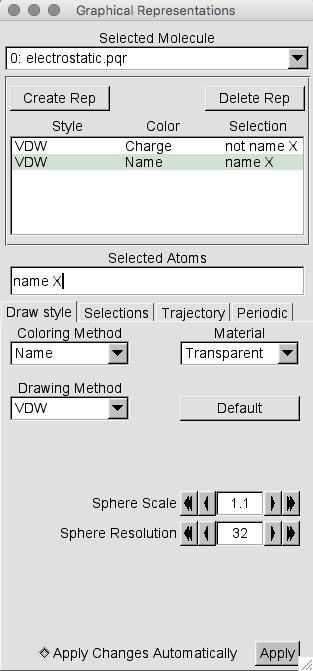
\includegraphics[width=\textwidth]{vmd_graph_rep_pqr}
    \caption{Graphics}
  \end{minipage}
  \hfill
  \begin{minipage}[b]{0.65\textwidth}
    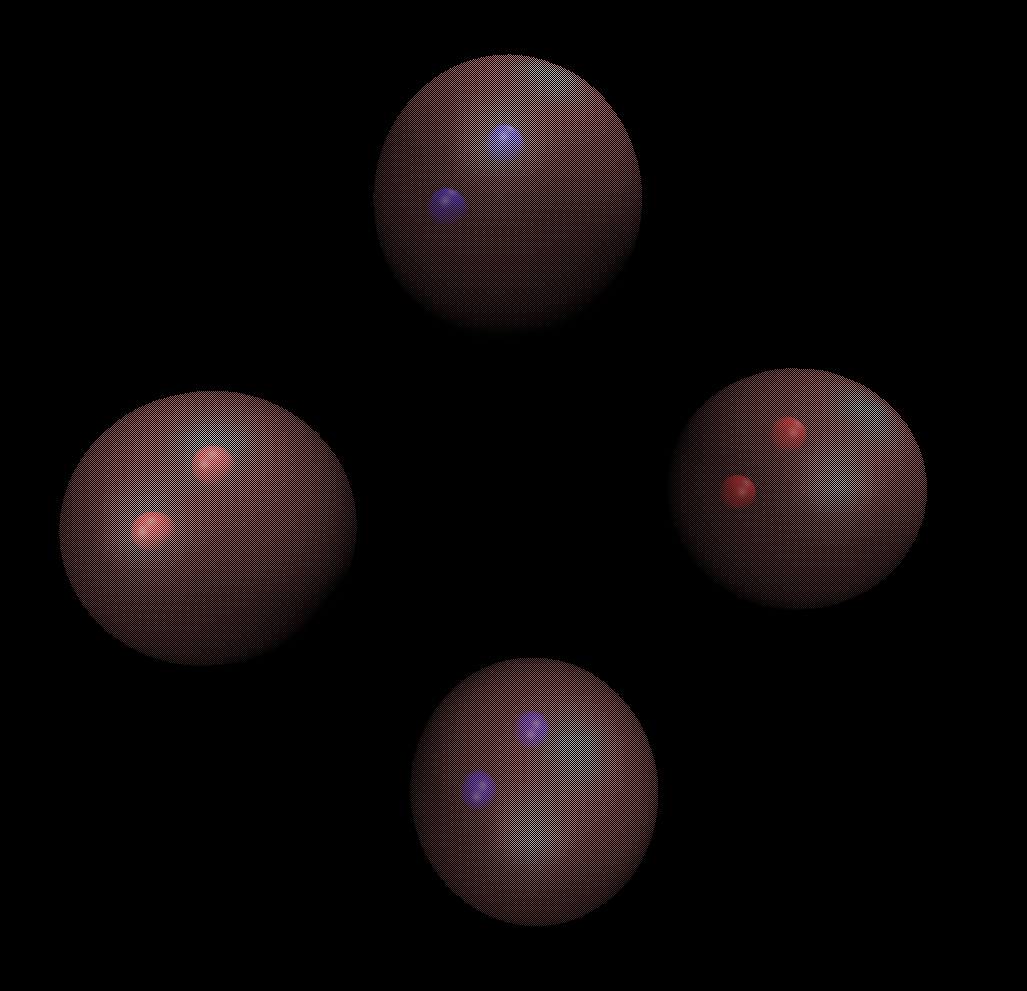
\includegraphics[width=\textwidth]{vmd_4sp}
    \caption{Final view}
  \end{minipage}
\end{figure}

\section{Viewing Electrostatics in VMD}

To load electrostatic results: File \textgreater \, New Molecule. In the window that appears, toggle the \textit{Load files for:} 
to select the currently loaded PQR file. Then select \textit{Browse} to find the location of the dx file. Once found, hit 
the \textit{Load} button and let the dx file load.

\begin{figure}[!htbp]
  \centering
  \begin{minipage}[b]{0.3\textwidth}
    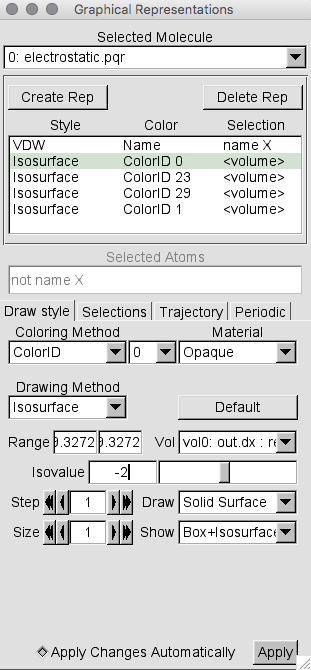
\includegraphics[width=\textwidth]{vmd_graph_rep_dx}
    \caption{DX Graphics}
  \end{minipage}
  \hfill
  \begin{minipage}[b]{0.65\textwidth}
    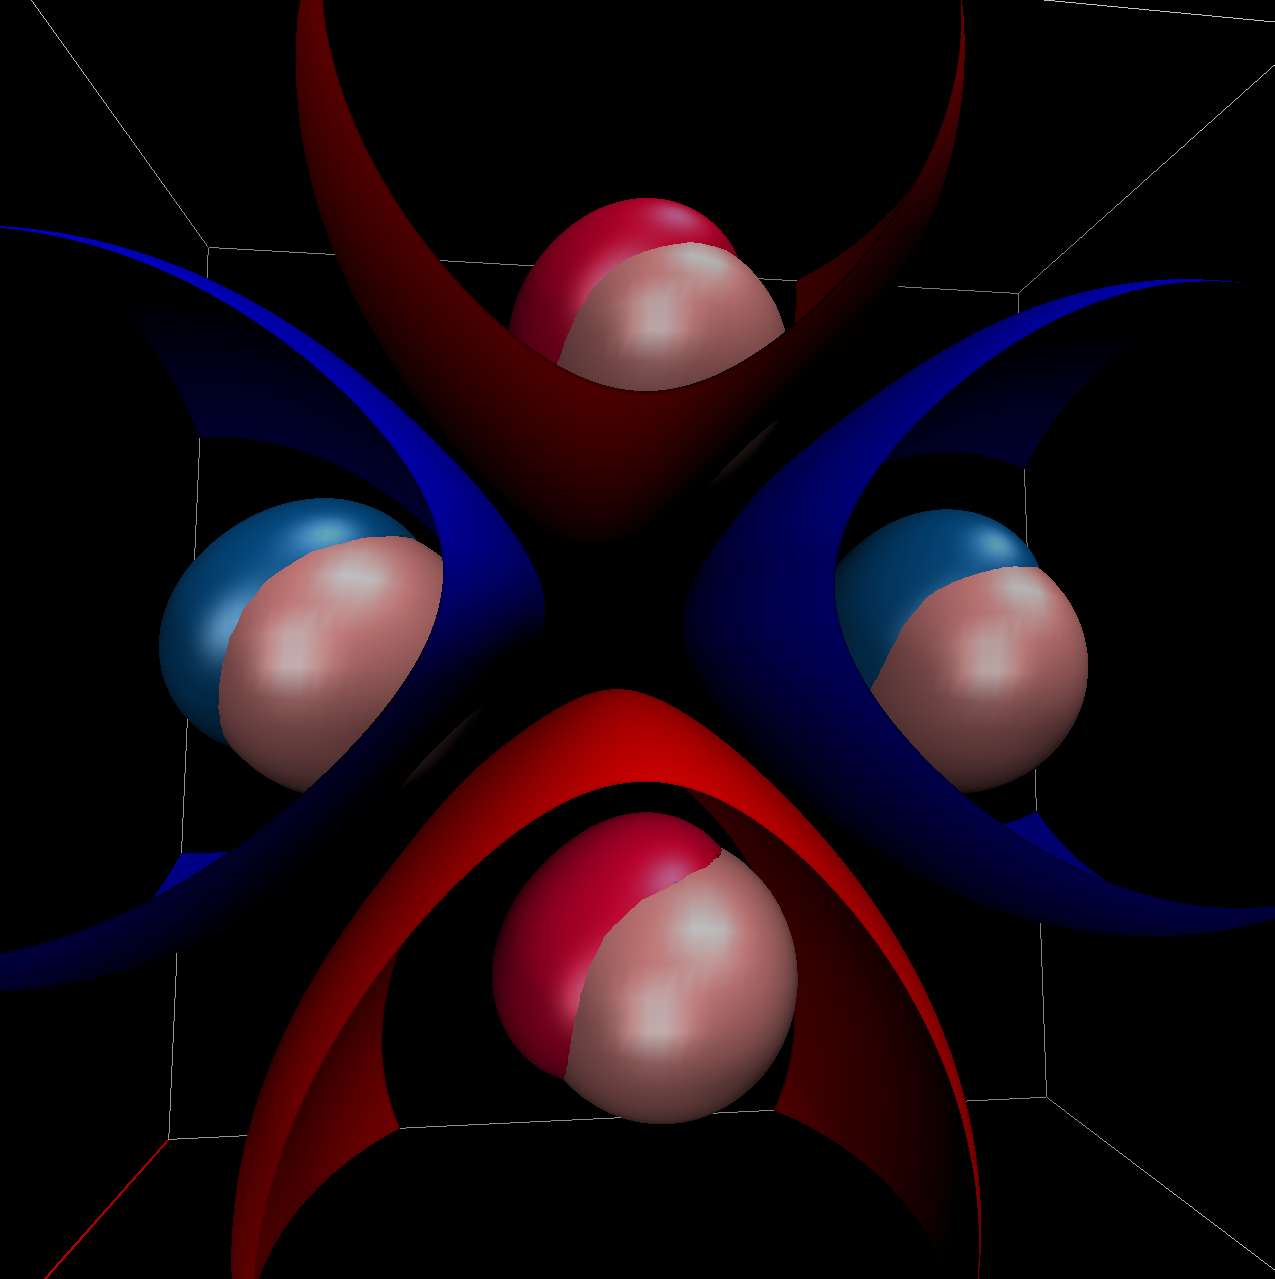
\includegraphics[width=\textwidth]{vmd_4sp_dx}
    \caption{DX representation}
  \end{minipage}
\end{figure}

 \clearpage

%\section{Mean First Passage Time (MFPT)}
%
%collect FPT from complete.dat
%\begin{lstlisting}[style = MyBash]
%	>> cat <yourpath>/complete.dat | awk '{print $7}' >  fpt.txt
%\end{lstlisting}
%run lognorm.py 
%\begin{lstlisting}[style = MyBash]
%	>> python lognorm.py  <yourpath>/fpt.txt
%\end{lstlisting}
%The final line of the output gives average and standard deviation for first passage times
%based on the lognormal probability distribution.
%The other lines output shape parameters describing the skew and kurtosis of the PDF
%It can also plot the histogram of FPT.
%
%
%To Do : get diffusion constant from fpt.txt as well


\section{2D ESP plots}
From the electrostatic option in PB-AM, a file is created with the following format: \\

\begin{lstlisting}[style = MyBash]
# Data from PBAM Electrostat run
# My runname is barnase.x.0.dat
units kT
grid 200 200 
axis x 0 
origin -51.2204 -51.2204
delta 0.512204 0.512204
maxmin 1.35396 0
   0.2352107     0.2360552     0.2368904     0.2377159
\end{lstlisting}

\medskip

In our \texttt{tools} directory we have provided a python script for plotting this potential.
Change filename within .py file, and the desired output name.
\begin{lstlisting}[style = MyBash]
>> python potential_plot
\end{lstlisting}

\medskip

creates a JPG file of the cross sectioned potential, like the one given below:

\begin{figure}[!htbp]
  \centering
    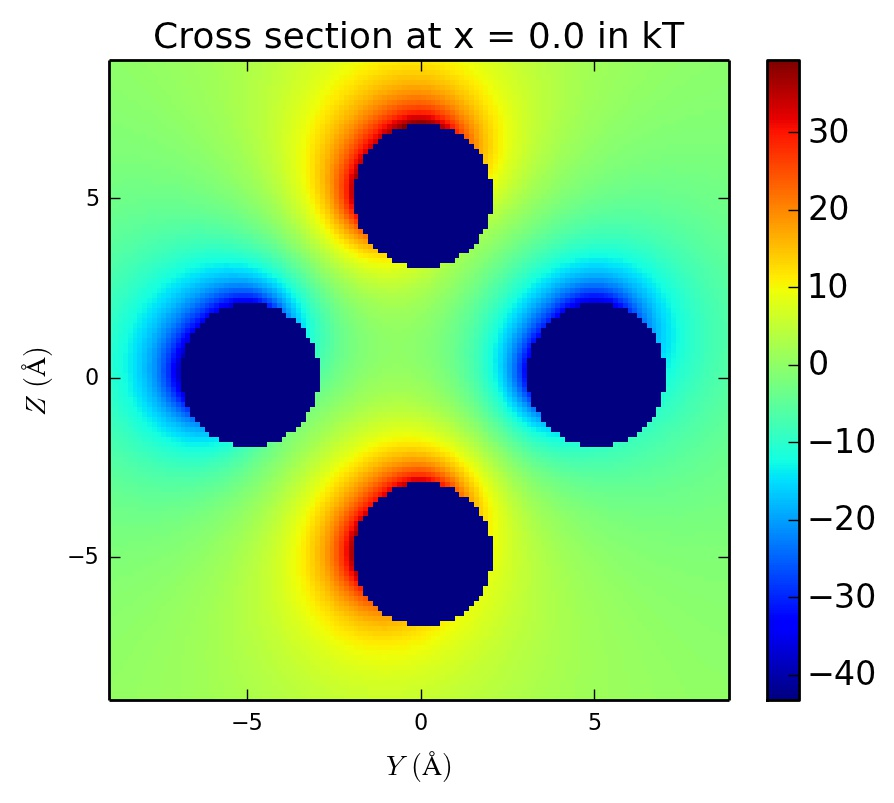
\includegraphics[scale=0.3]{pot_x_0}
    \caption{Potential plot}
\end{figure}

\section{3D ESP plots}
From the electrostatic option in PB-AM, a file is created with the following format: \\

\begin{lstlisting}[style = MyBash]
# Data from PBAM Electrostat run
# My runname is electro_map.out and units kT
grid 10 10 10
origin -4 -9 -9
delta 0.8 1.8 1.8
  0.00000   0.00000  -2.90000 -5.899581 
\end{lstlisting}

\medskip

In our \texttt{tools} directory we have provided a python script for plotting this potential.
Change filename within .py file, and the desired output name.
\begin{lstlisting}[style = MyBash]
>> python plot_3d_surf
\end{lstlisting}

\medskip

creates many JPG files of the cross sectioned potential, like the one given below:

\begin{figure}[!htbp]
  \centering
    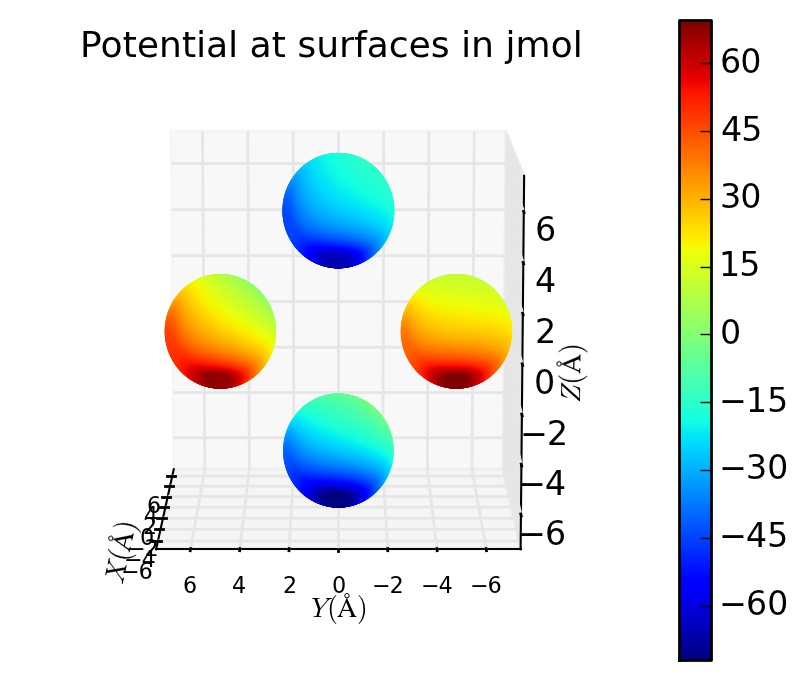
\includegraphics[scale=0.4]{4sp_surf}
    \caption{Molecule surface potential plot}
\end{figure}

	
%\section{Comparison of Displacement Due to Electrostatics versus Diffusion}	
%
%Because Brownian dynamics directly calculated displacements, 
%it is easier to compare relative displacements rather than relative forces.
%
%Separate the displacements due to Electrostatics and Diffusion into their own files.
%In the same directory as bdtest.out :
%\begin{lstlisting}[style = MyBash]
%	>> bash cfDisplacements.sh
%\end{lstlisting}
%Currently set to use only the final completed trajectory in bdtest.out
%This creates two files : dispES.out and dispRand.out
%In the same directory:
%\begin{lstlisting}[style = MyBash]
%	>> python avgDisp.py
%\end{lstlisting}
%This outputs the average displacement in Angstroms due to electrostatics and diffusion, in that order.
%
%
%
%\section{Length Scaling of FPT}
%
%How does the MFPT change with arbitrary choice of length scale?
%
%\begin{lstlisting}[style = MyBash]
%	>> bash lengthScale.sh
%\end{lstlisting}
%
%This script re-analyzes the trajectory for FPT with distances of 10, 20, ... \AA{}.





\chapter{Common Errors}

\section{Errors while reading input file}
Our file reader catches some errors, like files not exisiting or
being unable to open them. Look at the verbose stream of the
program to make sure all your flags are being caught, and check the
stream for errors as well.

\section{Segmentation Fault while reading input file}
Our file reader is not very robust.
Make sure there is only a single space between keywords and options.
Make sure that all options are specified for a given keyword.

\section{Initial configuration errors}
Many issues may arise if your molecules are overlapping, which is not allowed in the PB solvers' models.
The center of the molecule will be placed at the positions given by each XYZ file.
Check the printed out PQR file for the initial configuration, which you can load into VMD.
Try changing the xyz file(s).
This error may also appear if the box length specified with the pbc keyword is too small.
Try increasing the box length.












\phantomsection
\addcontentsline{toc}{chapter}{Bibliography}
\bibliographystyle{jacs}
\bibliography{pbsam}


\end{document}

